\section{Budget}


\subsection{Projected Attendance}
We project to have 450 student attendees and 150 professional attendees. We have based these projections on the attendance from previous years and on our central midwestern location. Additionally, this estimate allows us to create the most conservative budget possible and be prepared in the event that attendance is unusually high. A summary of the previous attendance is shown in Table \ref{table:attendance}.

\begin{table}[H]
\caption{Summary of Previous Attendance}
\label{table:attendance}
    \centering
    \begin{tabular}{cccccccccccc}
    \textbf{Host}& VCU & UF & UPitt & UWM & T. A\&M & Penn & MIT & UNLV & GIT & Mean ($\mu$) & Margin ($\frac{\sigma}{\sqrt{N}}$) \\
    \hline
    Students & 450 & 430 & 500 & 438 & 375 & 388 & 536 & 400 & 425 & 438 & $\approx$16 \\
    Professionals & 100 & 120 & 75 & 130 & 137 & 134 & 101 & 200 & 150 & 127 & $\approx$11\\
    \hline
    \end{tabular}
\end{table}
% =======================================================================================
% =======================================================================================
% =======================================================================================
% =======================================================================================
% Revenue Section
% =======================================================================================
% =======================================================================================
% =======================================================================================
% =======================================================================================

\subsection{Revenue}
We have compared the predicted and actual revenues from previous reports and used these to estimate our expected revenue. To maintain reasonable accuracy in the budget, we were financially conservative in our estimates to account for fluctuating economy and attendance numbers. Should our bid be selected, these conservative estimates will result in a smoother planning and execution process. We have also accounted for an estimated number of waived professional registration based on previous conferences. This  correlates to the number of waived fees given in our expected tier sponsorship figures and also factors in discounts to speakers, panelists, and workshop instructors. \\

\clearpage
\begin{table}[H]
\centering
\caption*{\textbf{Attendance Revenue}}
\begin{tabular}{|c|c|c|c|}
\hline
    \textbf{Item} & \textbf{Quantity} & \textbf{Cost} & \textbf{Subtotal}	\\ 
\hline
	Student			&	450	&	\$40	&	\$18,000						\\
	Professional	&	150	& 	\$250	&	\$37,500						\\
	Waived			&	60	& 	-\$250	&	-\$15,000						\\
\hline
	\multicolumn{3}{|r|}{\textbf{Attendance Total:}}	&	\$40,500		\\
\hline
\end{tabular}
\end{table}

% \vspace{10mm}

\begin{table}[H]
\centering
\caption*{\textbf{Sponsorship Revenue}}
\begin{tabular}{|c|c|c|c|}
\hline
    \textbf{Package} & \textbf{Quantity} & \textbf{Cost} & \textbf{Subtotal}	\\ 
\hline
	World Savior	&	1	&	\$30,000	&	\$30,000						\\
	National Hero	&	3	& 	\$15,000	&	\$45,000						\\
	Local Prodigy	&	5	& 	\$10,000	&	\$50,000						\\
	Lifesaver		&	6	& 	\$5,000		&	\$30,000						\\
	Exhibitor+		&	3	& 	\$3,500		&	\$10,500						\\
	Exhibitor		&	5	& 	\$2,500		&	\$12,500						\\
	Good Samaritan	&	10	& 	\$1,500		&	\$15,000						\\
	Contributor		&	8	& 	\$1,000		&	\$8,000							\\
\hline
	\multicolumn{3}{|r|}{\textbf{Sponsors Total:}}	&	\$201,000				\\
\hline
\end{tabular}
\end{table}

% \vspace{10mm}

\begin{table}[H]
\centering
\begin{tabular}{|c|}
\hline
    \textbf{Total Revenue: \$241,500}\\ 
\hline
\end{tabular}
\end{table}

% =======================================================================================
% =======================================================================================
% =======================================================================================
% =======================================================================================
% Expenses Section
% =======================================================================================
% =======================================================================================
% =======================================================================================
% =======================================================================================

\subsection{Expenses}
A conservative breakdown of conference expenses is outlined in Table \ref{table:budget} on page \pageref{table:budget}. All rooms hosted in the Union are provided to registered student organizations (such as ANS-UIUC) free of charge. This allows us to save significantly on event space. Meals catered through the University catering service reflect a 6.25\% sales tax in the total cost which is not represented in the unit cost. Gratuity is neglected because it is forbidden under the catering service’s policies, allowing us to save 20\% gratuity on meals. 
Under our most conservative estimates for budget and revenue, the spending margin is found to be 6.8\%. While this margin is tight, we feel this is justified as several costs in the expenses, such as reimbursements, are left significantly inflated as compared with previous years. Adopting previous years’ estimates of \$60,000 for travel reimbursements leaves a spending margin of 21.6\%, matching that of the most austere contingency plans provided in previous years. 
Assuming maximum expenses and an attendance of 450 students, the total cost per student is estimated at \$501.63. This number also includes the travel reimbursement, which was intentionally set to be considerably more generous than previous years to make the budget more conservative. Assuming every student traveled here with the avereage cost of flights from Table \ref{table:airfare}, our current travel reimbursement package would cover 76.8\% of the accumulated costs. Neglecting the cost of travel reimbursements, the average cost per student falls to \$276.63, at or below that estimated for previous years. In Appendix \ref{appendix:quotes} on page \pageref{appendix:quotes} we included quotes where possible.

% \hspace{-1.1cm}
\begin{table}[H]
    \caption{Budget Expenses}
    \label{table:budget}
    \makebox[\linewidth]{
        \begin{tabular}{|clcrccccr|}
    
        \hline
         & \multicolumn{1}{c}{\textbf{Item}} & \multicolumn{1}{c}{\textbf{Priority}} & \multicolumn{1}{c}{\textbf{Cost Per Unit}} & \multicolumn{1}{c}{\textbf{Thursday}} & \multicolumn{1}{c}{\textbf{Friday}} & \multicolumn{1}{c}{\textbf{Saturday}} & \multicolumn{1}{c}{\textbf{General}} & \multicolumn{1}{c}{\textbf{Total Cost}}\\     \hline\hline
         \multirow{10}{*}{\STAB{\rotatebox[origin=c]{90}{\textbf{Facilities}}}}
         & Technical Session AV      & I                         & $\$$ 13.80                & 1                         & 6                        & 6                         & -                         & $\$$179.40               \\
         & Technical Session Rooms   & I                         & $\$$ 0.00                 & -                         &  -                       &  -                        &  1                        & $\$$0.00                 \\
         & Panel AV                  & I                         & $\$$ 17.80                & -                         &   2                      &   2                       &   -                       & $\$$71.20                \\ 
         & Panel Rooms               & I                         & $\$$ 0.00                 & -                         &    -                     &    -                      &    1                      & $\$$0.00                 \\
         & Workshop AV               & I                         & $\$$ 17.80                & 2                         &     -                    &     -                     &     -                     & $\$$35.60                \\
         & Workshop Rooms            & I                         & $\$$ 0.00                 &  -                        &      -                   &      -                    &      1                    & $\$$0.00                 \\ 
         & Dinner Room (Ihotel)      & I                         & $\$$ 4,000.00             &   -                       &       -                  &       1                   &       -                   & $\$$4,000.00             \\
         & Dinner AV (Ihotel)        & I                         & $\$$ 0.00                 &    -                      &        -                 &        1                  &        -                  & $\$$0.00                 \\
         & Dinner Room (Garden Hotel)& I                         & $\$$ 4,000.00             &     1                     &         1                &         -                 &         -                 & $\$$8,000.00             \\ 
         & Dinner AV (Garden Hotel)  & I                         & $\$$ 0.00                 &      1                    &          1               &          -                &          -                & $\$$0.00                 \\ \hline
         &                           &                           &                           &                           &\multicolumn{3}{r}{Facilities Subtotal:}     & $\$$12,286.20            \\ \hline\hline
         \multirow{5}{*}{\STAB{\rotatebox[origin=c]{90}{\textbf{Transport}}}}
         & Shuttles From Hotel       & I                         & $\$$ 1,000.00             & 4                         & 4                        & 4                         & -                         & $\$$12,000.00            \\
         & Ihotel Dinner             & I                         & $\$$ 875.00               & -                         &  -                       &  4                        &  -                        & $\$$3,500.00             \\
         & Brewery/Starfire Tours    & II                        & $\$$ 875.00               & 1                         &   -                      &   -                       &   -                       & $\$$875.00               \\ 
         & Clinton Tour              & II                        & $\$$ 875.00               & 1                         &    -                     &    -                      &    -                      & $\$$875.00               \\
         & Argonne Tour              & II                        & $\$$ 875.00               & 1                         &     -                    &     -                     &     -                     & $\$$875.00               \\ \hline
         &                           &                           &                           &                           &\multicolumn{3}{r}{Transport Subtotal:}      & $\$$18,125.00            \\ \hline\hline
         \multirow{5}{*}{\STAB{\rotatebox[origin=c]{90}{\textbf{Food}}}}
         & Coffee/Tea                & III                       & $\$$ 1.95                 & -                         & 600                      & 600                       & -                         & $\$$2,486.25             \\
         & Garden Hotel Dinners*     & II                        & $\$$ 36.50                & 600                       & 600                      &  -                        &  -                        & $\$$46,537.50            \\
         & Ihotel Dinner             & II                        & $\$$ 27.50                & -                         &   -                      &   600                     &   -                       & $\$$17,531.25            \\ 
         & Dinner Cash Bars          & III                       & $\$$ 336.00               & 1                         &    1                     &    1                      &    -                      & $\$$1,071.00             \\
         & SSC Lunches               & II                        & $\$$ 16.50                & -                         &     -                    &     150                   &     -                     & $\$$2,629.69             \\ \hline
         &                           &                           &                           &                           &\multicolumn{3}{r}{Food Subtotal:}           & $\$$70,255.69            \\ \hline\hline
         \multirow{5}{*}{\STAB{\rotatebox[origin=c]{90}{\textbf{Socials}}}}
         & Ice Skating               & III                       & $\$$ 240.00               & 2                         & -                        & -                         & -                         & $\$$480.00               \\
         & Illini Rec Room           & III                       & $\$$ 490.00               &  -                        & 2                        &  -                        &  -                        & $\$$982.00               \\
         & Memorial Stadium Club 77  & III                       & $\$$ 2,000.00             & -                         &   -                      &   1                       &   -                       & $\$$2,000.00             \\ 
         & Club 77 Tab               & IV                        & $\$$ 3,000.00             & -                         &    -                     &    1                      &    -                      & $\$$3,000.00             \\
         & Guido's Tab               & IV                        & $\$$ 3,000.00             & -                         &     1                    &     -                     &     -                     & $\$$3,000.00             \\ \hline
         &                           &                           &                           &                           &\multicolumn{3}{r}{Socials Subtotal:}        & $\$$9,462.00             \\ \hline\hline
         \multirow{7}{*}{\STAB{\rotatebox[origin=c]{90}{\textbf{Miscellaneous}}}}
         & Conference Programs       & I                         & $\$$ 2,133.90             & -                         & -                        & -                         & 1                         & $\$$2,133.90             \\
         & Lanyards                  & I                         & $\$$ 2.54                 &  -                        & -                        &  -                        &  600                      & $\$$1,524.00             \\
         & Award Certificates        & III                       & $\$$ 2.50                 & -                         &   -                      &   50                      &   -                       & $\$$125.00               \\ 
         & Poster Session Prizes     & III                       & $\$$ 100.00               & -                         &    -                     &    3                      &    -                      & $\$$300.00               \\
         & Swag                      & IV                        & $\$$ 10,000.00            & -                         &     -                    &     -                     &     1                     & $\$$10,000.00            \\ 
         & Brewery Tour              & IV                        & $\$$ 5.00                 & 45                        &     -                    &     -                     &     -                     & $\$$275.00               \\
         & Travel Reimbursements     & I                         & $\$$ 225.00               &  -                        &     -                    &                           &  450                      & $\$$101,250.00           \\ \hline
         &                           &                           &                           &                           &\multicolumn{3}{r}{Miscellaneous Subtotal:}                                       & $\$$126,857.90           \\ \hline\hline
         &                           &                           &                           &                           &                          &                           &                           &                          \\
         &                           &                           &                           &                           &\multicolumn{3}{r}{Grand Total:}                                                  & $\$$225,734.79           \\
         &                           &                           &                           &                           &                          &                           &                           &                          \\ \hline
    \end{tabular}}
\end{table}

\subsection{Financial Contingency}


\begin{table}[H]
    \caption{Budget Cuts}
    \label{table:cuts}
    \centering
    \makebox[0.65\linewidth]{\begin{tabular}{lrrr}
      \hline\hline
      \multicolumn{1}{l}{Level of Cuts Made} & \multicolumn{1}{c}{Amount Saved} & \multicolumn{1}{c}{Grand Total} & \multicolumn{1}{c}{\% of Max Revenue} \\ \hline\hline 
      Priority IV Cuts Made & $\$$9,346.00 & $\$$216,388.79 & 10.4\% \\
      III and IV Cuts Made & $\$$22,987.25 &$\$$198,747.54 & 17.4\% \\
      II, III, and IV Cuts Made & $\$$49,053.19 & $\$$176,681.60 & 26.56\% \\
      \hline
    \end{tabular}}
\end{table}

The budget is structured with priority levels outlining the order of cuts, should they be necessary. Priority I expenses are not subject to cuts under any circumstances as they are considered necessities for hosting the conference. Cuts will be made first to reduce most priority IV expenses by half, preserving events while still saving money. Priority III cuts mean eliminating all priority IV expenses and either elimination of, or reduction of the duration of social events by half. Priority II cuts entail complete elimination of social event expenses, along with elimination of tour expenses and reduction of dinner costs through cheaper buffet options and desserts. The expenditure savings from these cuts are outlined in Table \ref{table:cuts}. While this contingency plan does not consider cuts to the reimbursement funds, this could be reconsidered if necessary, since reimbursements were set aside at a level nearly double that of previous conferences. 

\subsection{Sponsorship and Fundraising}
The sponsorship breakdown for our conference pulls from averages of sponsorship 
packages in the last several conferences, with four main tiers that tie into the conference theme for the largest representation in the conference and visibility in the career fair, socials, sessions, technical, and meals as well as in conference shirts and attendee bags. Using two tiers for an exhibitor package allows for a platform for DOE national laboratories to participate, with the higher tier having logo representation on shirts as well as the opportunity to sponsor a coffee break or lunch \& learn session. Lastly, two packages are left to benefactors who are recognized in the conference program and represent the anticipated support from ANS divisions or local industry or University of Illinois contributors (or some generous contributions from out-of-state companies!). 

% \vspace{1cm}

\begin{figure}[H]
	\centering
	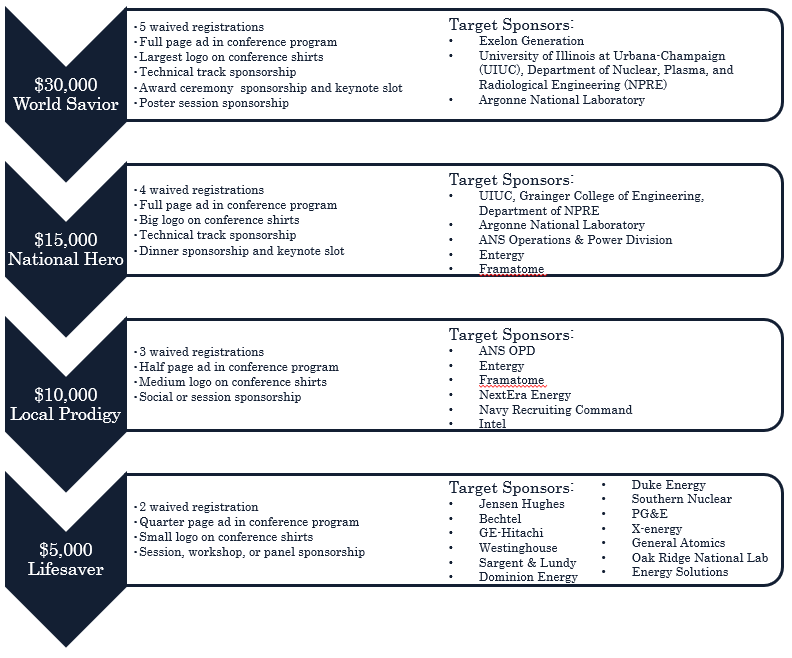
\includegraphics[width=0.85\textwidth]{sponsors1.png}	
\end{figure} 

\begin{figure}[H]
	\centering
	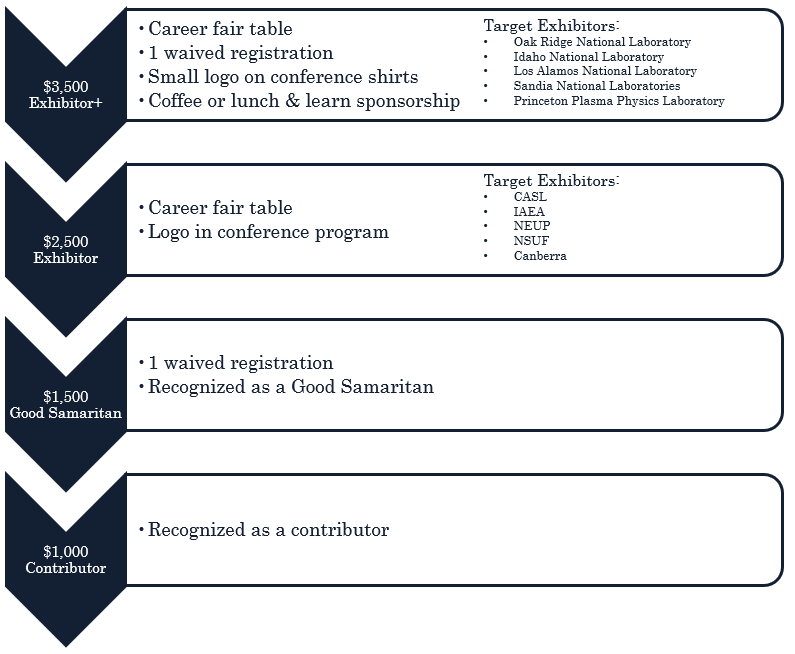
\includegraphics[width=0.85\textwidth]{sponsors2.png}	
\end{figure} 

\subsection{Banking}

In order to properly handle all of the conference expenses, two accounts will be used. One account will be with the national ANS headquarters, and the second will be a local checking account through Busey Bank. Our student section currently holds a checking account with Busey Bank and has developed a working relationship with them. Similar to previous conferences, the national ANS account will be the primary account due to their previous experience in handling conference funds and their 501(c)(3) tax exemption status. Although an account with the national ANS organization is currently not maintained by the UIUC local chapter, should this bid be selected, the opening of an account would happen almost immediately. An established local checking account with Busey Bank allows for convenience when using them as a secondary account. The student section account has been maintained for a number of years, allowing for adequate knowledge of Busey’s policies and a stable relationship to be established with the local branch. A new account would be opened, such that the student chapter funds and the conference funds are completely separate and require different oversight. This account will be used for small expenses that can occur during the conference. Although the ANS-managed account could be used for such purposes, the presence of a local branch allows for more flexibility if a purchase becomes time sensitive. Should the additional Busey Bank account be unobtainable, an account would be established with Chase instead. If ANS National desires to manage all funds, accommodations will be made to consolidate the funds.

\subsubsection{Financial Oversight}
Financial integrity must be maintained when providing a conference of this size. To do so, diligent oversight will be practiced for all transactions related to the conference. Expense requests will be required for all transactions. These requests must carefully outline the reason for the purchase and the total cost. If the purchase is reoccuring, automation will be required at the time of request. These requests will require the approval of both conference chairs in addition to the financial director. Only the conference chairs and the financial director will have authority, assuming the previously mentioned permission, to complete transactions on the Busey Bank account. To ensure transparency, the financial director will update a public record containing all transactions. 

\subsection{Cost of Attendance and Student Reimbursement}
The cost of attending the student conference, per student, varies among schools 
and is highly dependent on distance from UIUC and the preferred mode of travel. 
We will assume that minimizing cost is a priority for schools, thus number of 
persons per hotel room is assumed to be double the number of beds. The 
University of Illinois is a 2.5 hour drive from one of the largest airports in 
the world, O'Hare International Airport. There is also a small airport located 
just 15 minutes outside of campus which has regular flights to Chicago O'Hare 
(ORD), Dallas/Fort Worth (DFW), and Charlotte (CLT). While some students may 
wish to make use of the convenience of the local airport, in general the most 
economic method of arriving in Champaign is by first flying to O’Hare and then 
busing. The average cost of this trip comes out to be \$293 as shown in Table  
\ref{table:airfare}. Adding this to the registration and lodging costs (see 
Table \ref{table:hotels}) for four nights (as students often arrive Wednesday 
evening) and assuming four students per room, \textbf{the total cost of attendance for 
each student comes out to an average of \$447.} The travel reimbursement is 
meant to help mitigate some or most of the costs for students coming to this 
conference to encourage future attendance at other conferences.

% Jeremy's budget plan

\subsection{Student Travel Reimbursement Procedure}
The procedure for student travel reimbursement will require each section send via email all acquired expenses in their travels and lodging for this conference. Each chapter will be required to send us:
\begin{enumerate}
    \item The number of students that attended.
    \item The number of hotel rooms reserved.
    \item The location of the hotel rooms.
    \item Modes of transportation
    \item Parking costs (excluding airport reserved parking).
    \item Receipts for all purchases will be required for all submitted purchases.
\end{enumerate}
A form will be emailed to each of the chapter presidents for their section to fill out and attach the appropriate receipts. We will require that the form along with the necessary receipts be submitted via email to the Finance Director in one PDF, two weeks after the Sunday following the conference. The Finance Chair will review all of the submitted documents for any corrections that need to be made. Any section that needs to make corrections to their reimbursement form will be emailed the following Tuesday. The reimbursement form must be re-submitted to us by that Friday. Once all the sections have their forms submitted to us we will turn in our master list to ANS National for reimbursement distributions. Checks will be mailed to each of the chapter presidents or a selected representative for the chapter.
